\chapter{Introduction}
\label{ch:intro}

\section{Context and motivation}
\label{sec:motivation}

Public blockchains commonly authorise transactions with the Elliptic Curve Digital
Signature Algorithm (ECDSA) or Schnorr. Their security relies on the hardness of the
elliptic-curve discrete logarithm problem, which Shor's algorithm solves in polynomial
time on a sufficiently large quantum computer \cite{shor1999polynomial}, allowing an
adversary to forge signatures and spend other users' funds. A published 2026 resource
estimate addresses that curve directly (\cref{fig:whynow}). A
chain cannot treat that as distant: its record is permanent, so a break reaches keys
already exposed, and changing how it verifies signatures requires a coordinated
consensus-rule change, not merely a local software update. ``Post-quantum'' (PQ)
cryptography replaces this assumption with
problems believed hard even for quantum computers, such as those over lattices.

The U.S. National Institute of Standards and Technology (NIST) has standardised
\emph{basic} PQ signatures, notably ML-DSA (the Module-Lattice-Based Digital Signature
Algorithm), derived from CRYSTALS-Dilithium
\cite{1274601,ducas2018crystals}. A basic signature authenticates a message and nothing
more. Blockchains, however, depend on \emph{exotic} signatures that add functionality
on top of a basic scheme: multi-signatures, aggregate signatures, threshold
signatures, and \emph{adaptor signatures}. A recent survey documents that, while basic PQ signatures are
maturing, their exotic counterparts remain unevenly served by practical implementations
in blockchain settings \cite{buser2023survey}. Turning one such paper design into a
tested, measured artefact is the problem this project addresses.

\begin{figure}[htbp]
  \centering
  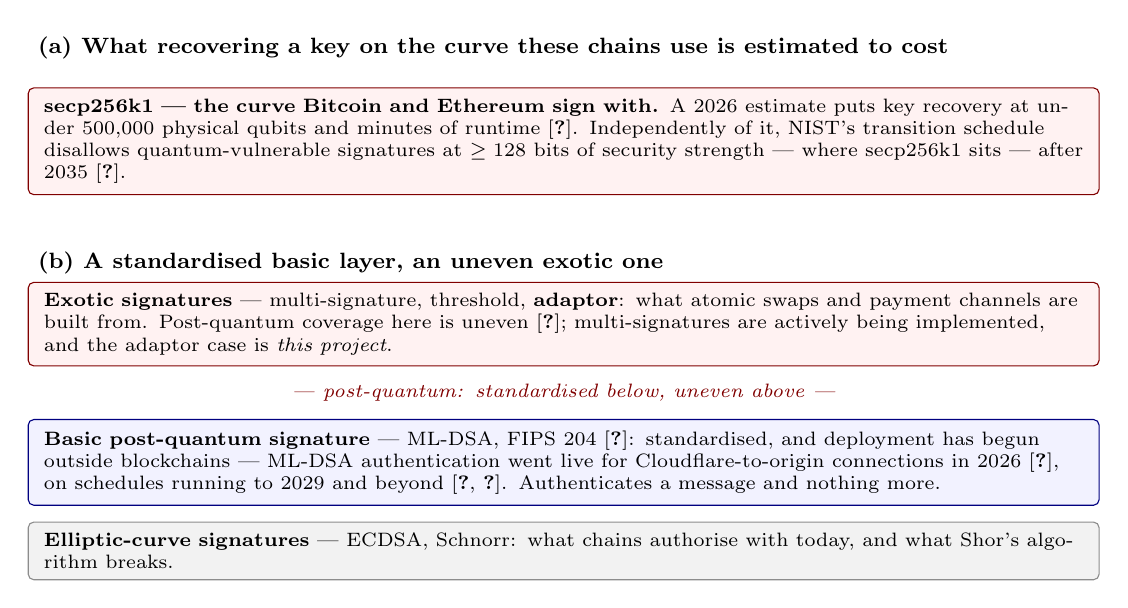
\begin{tikzpicture}[
      font=\scriptsize,
      ttl/.style={font=\footnotesize\bfseries, anchor=west},
      %% (an "est" style for the old three-column timeline lived here until the panel
      %% was rebuilt on 2026-08-27; it is referenced nowhere now)
      tier/.style={draw, rounded corners=2pt, align=left, text width=132mm,
                   inner xsep=2mm, inner ysep=1.4mm, anchor=north},
      gap/.style={font=\scriptsize\itshape, anchor=north, align=center,
                  text width=132mm}]

    %% Geometry: EVERY box is centred on x = 0 and the picture stays inside \textwidth
    %% (145mm).  Tier boxes span [-68mm, 68mm] (132mm text + 2mm inner xsep either
    %% side), and both panel titles are left-anchored at -68mm to match that edge.
    %% Keep it symmetric -- mixing left-anchored coordinates for (a) with centred ones
    %% for (b) once put the two halves on different axes and overran the text block.
    %% Vertical placement is RELATIVE (each row hangs off the previous one), so a row
    %% may grow in height without being edited into a collision.

    %% ---- (a) the estimated cost of breaking THE CHAINS' OWN curve ----
    %% Rebuilt 2026-08-27 (Meeting 12).  The earlier version was a three-dot timeline,
    %% two dots of which were RSA-2048; the supervisor read that as arguing from a
    %% target neither chain uses ("Bitcoin and also Ethereum, they are not using RSA")
    %% and asked for something "much closer to Bitcoin, or to blockchain itself".  The
    %% RSA figures are therefore REMOVED, not demoted.  Two consequences, both wanted:
    %% the panel now argues at secp256k1 only, and with no second target present there
    %% is no pair to divide, so the across-targets misreading is structurally gone.
    %% If any RSA figure is ever restored, the caption's separation caveat must come
    %% back with it -- and \cite{gidney2021factoring,gidney2025factoring} with it.
    %% WORDING: "the CURVE these chains use", never "the signature" -- they share
    %% secp256k1, not one scheme (Bitcoin has ECDSA and Schnorr).
    \node[ttl] at (-68mm,0) {(a) What recovering a key on the curve these chains use is
        estimated to cost};
    \node[tier, fill=red!5, draw=red!50!black] (pri) at (0mm,-5mm)
      {\textbf{secp256k1 --- the curve Bitcoin and Ethereum sign with.} A 2026 estimate
       puts key recovery at under 500{,}000 physical qubits and minutes of runtime
       \cite{babbush2026securing}. Independently of it, NIST's transition schedule
       disallows quantum-vulnerable signatures at $\ge 128$ bits of security strength
       --- where secp256k1 sits --- after 2035 \cite{nistir8547}.};
    \coordinate (bTop) at ([yshift=-6mm]pri.south);

    %% ---- (b) a standardised basic layer, an uneven exotic one ----
    %% NOT "standardisation stops": the cited claim is about the availability of
    %% practical IMPLEMENTATIONS, and multi-signatures are actively being built.
    %% Anchored to (a)'s last row via bTop, NOT to an absolute y: (a) may grow without
    %% the two halves colliding.
    \node[ttl, anchor=north west] at ([xshift=-68mm]bTop)
      {(b) A standardised basic layer, an uneven exotic one};
    \node[tier, fill=red!5, draw=red!50!black] (ex) at ([yshift=-5mm]bTop)
      {\textbf{Exotic signatures} --- multi-signature, threshold, \textbf{adaptor}:
       what atomic swaps and payment channels are built from. Post-quantum coverage
       here is uneven \cite{buser2023survey}; multi-signatures are actively being
       implemented, and the adaptor case is \emph{this project}.};
    \node[gap, red!50!black] (gp) at ([yshift=-1mm]ex.south)
      {--- post-quantum: standardised below, uneven above ---};
    %% NOT "being adopted now" unevidenced (the wording here until 2026-08-27, and the
    %% thing the supervisor asked for twice): deployment outside blockchains is CITED,
    %% and the live one is signature AUTHENTICATION on Cloudflare-to-origin connections
    %% -- never the public web PKI, where no post-quantum certificate was in use in 2025.
    \node[tier, fill=blue!5, draw=blue!50!black] (ba) at ([yshift=-1mm]gp.south)
      {\textbf{Basic post-quantum signature} --- ML-DSA, FIPS~204 \cite{1274601}:
       standardised, and deployment has begun outside blockchains --- ML-DSA
       authentication went live for Cloudflare-to-origin connections in 2026
       \cite{valenta2026pqauth}, on schedules running to 2029 and beyond
       \cite{cloudflare2026pqroadmap,nistir8547}. Authenticates a message and nothing
       more.};
    \node[tier, fill=black!5, draw=black!45] (ec) at ([yshift=-2mm]ba.south)
      {\textbf{Elliptic-curve signatures} --- ECDSA, Schnorr: what chains authorise
       with today, and what Shor's algorithm breaks.};
  \end{tikzpicture}
  \caption[Why now, and where the gap is]{Why the problem is timely, and where this
  project sits within it. \textbf{(a)} The case is made at the curve these chains
  actually sign with, secp256k1, rather than at a reference target neither of them
  uses. This is an estimate, for hardware nobody has built: what such work reports is
  the \emph{estimated cost of the attack}, not a calendar. The deadline beside it is
  independent of that estimate --- a policy schedule, which binds regardless of when
  the hardware arrives. \textbf{(b)} A
  blockchain does not rest on one signature but on a stack of them. The basic layer,
  which authenticates a message and nothing more, is standardised and being adopted;
  the functionality chains actually depend on lives in the exotic layer above it, where
  practical post-quantum coverage is uneven. That migration is not a blockchain concern
  alone, and it has run ahead on encryption: post-quantum key agreement already carried
  the majority of human traffic on one major network while no public post-quantum
  certificate was yet in use \cite{westerbaan2025pqinternet}, and post-quantum
  \emph{signatures} followed later --- ML-DSA authentication went live there for
  connections to origin servers in July 2026 \cite{valenta2026pqauth}, with full
  coverage targeted for 2029 \cite{cloudflare2026pqroadmap}. The basic signature layer
  is therefore the current frontier outside blockchains too. This dissertation addresses one scheme in
  that layer, the adaptor signature.}
  \label{fig:whynow}
\end{figure}

This dissertation focuses on the \emph{adaptor signature}, which ties the act of
publishing a valid signature to the simultaneous revelation of a secret witness
\cite{poelstra2017,aumayr2021generalized}. That property makes adaptor signatures useful
for scriptless blockchain protocols. In an atomic swap, revealing the witness on one leg
provides what is needed to complete the other, letting two parties exchange assets across
chains without a trusted intermediary (\cref{fig:swapidea}). They have also been applied to payment-channel
networks, linking conditional off-chain updates through the same
witness mechanism. Because the condition is embedded in the signature rather than
published separately, the result verifies as an ordinary signature and the condition need
not appear as a separate on-chain script \cite{esgin2020post,buser2023survey}. Existing
classical constructions rely largely on discrete-logarithm assumptions and so are not
post-quantum secure, while practical post-quantum implementations remain limited. That
combination --- important blockchain applications, and an implementation gap --- is why
the adaptor signature was selected from the exotic-signature family.

% MOVED HERE FROM ch:results 2026-08-27, after Meeting 12.  Wang reviewed the REPORT with
% the PDF on screen and named the adaptor motivation as the one substantive shortfall --
% "why is it important for blockchains?", "we need some concrete motivation, the concrete
% examples", "you should at least give some introduction regarding applications of the
% adaptor signature".  This figure is exactly that concrete example, so it belongs beside
% the claim it makes concrete rather than three chapters later.
%
% This does NOT disturb Meeting 10's ruling, which has two parts: Fig. 3.5 (fig:swapflow)
% is ACCEPTED and stays where it is -- it does, in ch:results -- and a simpler diagram goes
% "before it, where the application is introduced".  Both still hold: Chapter 1 precedes
% Chapter 3, and the application is now introduced HERE.  When M10 was given, it was
% introduced only in ch:results, because this chapter carried no atomic-swap material at
% all; that material is the Meeting-12 expansion above.
%
% Word cost is nil: a figure body and its caption are both excluded from the count, and the
% \cref added above is paid for by the one dropped from ch:results.
%
% PARTY NAMING IS SETTLED (2026-08-16) -- do not "fix" it either way.  The subscripts stay:
% this figure is the ONLY place Alice/Bob is tied to the u_1/u_2 the technical chapters use,
% and dropping them reintroduces exactly the inconsistency that decision removed.  What did
% not survive the move is the caption's old "used from here on", which was true when this
% figure sat in ch:results and is false here; the tie is restated neutrally instead.
%
% REDRAWN 2026-08-27 and the redraw MUST survive any future edit.  An earlier version drew
% one arrow from Alice to Bob and another back, with the ledgers reduced to words ON those
% arrows -- so the picture invited the reading that a coin travels from one chain to the
% other, which is false, and left the caption denying what the drawing showed.  The ledgers
% are the drawn objects now: each payment is a transaction sitting INSIDE its own lane.  Do
% not reintroduce a party-to-party coin arrow.  Absolute coordinates only -- no calc.
\begin{figure}[htbp]
  \centering
  \begin{tikzpicture}[
      font=\small,
      party/.style={draw, rounded corners=3pt, align=center, minimum width=50mm,
                    minimum height=10mm, line width=0.6pt},
      lane/.style={draw, rounded corners=3pt, align=center, minimum width=120mm,
                   inner ysep=1.6mm, line width=0.6pt},
      lbl/.style={font=\footnotesize\itshape, align=center},
      >={Stealth[]}]

    \node[party, fill=orange!12, draw=orange!60!black] (a) at (30mm,0mm)
      {Alice $(u_1)$};
    \node[party, fill=blue!10, draw=blue!60!black] (b) at (90mm,0mm)
      {Bob $(u_2)$};

    \node[lane, fill=orange!8, draw=orange!60!black] (c1) at (60mm,-14mm)
      {\textbf{Chain~A} --- where Alice's coin lives\\
       $\mathrm{tx}_1$: Alice's coin $\rightarrow$ an address \emph{Bob} owns. Settles
       \emph{here}, as an ordinary payment.};

    % The link is drawn as two arrows FLANKING the label, so the label never covers the
    % thing it is labelling, and it is wrapped to stay inside the lane width.
    \draw[<->, dashed, line width=0.9pt, green!40!black] (12mm,-19.5mm) -- (12mm,-32.5mm);
    \draw[<->, dashed, line width=0.9pt, green!40!black] (108mm,-19.5mm) -- (108mm,-32.5mm);
    \node[lbl, green!35!black, text width=104mm] at (60mm,-26mm)
      {one settlement reveals the secret that unlocks the other\\
       --- the coins never cross chains};

    \node[lane, fill=blue!8, draw=blue!60!black] (c2) at (60mm,-38mm)
      {\textbf{Chain~B} --- where Bob's coin lives\\
       $\mathrm{tx}_2$: Bob's coin $\rightarrow$ an address \emph{Alice} owns. Settles
       \emph{here}, as an ordinary payment.};

    \node[draw, rounded corners=2pt, fill=green!8, draw=green!45!black,
          align=center, font=\footnotesize, minimum width=120mm] at (60mm,-50mm)
      {\textbf{Either both transactions settle, or neither does.}\\
       No centralised exchange, and nobody trusted to hold both sides.};
  \end{tikzpicture}
  \caption[An atomic swap, in outline]{What an atomic swap is for, before any
  cryptography --- one concrete blockchain application of adaptor signatures. Two parties
  want to trade coins that live on two different chains, and the danger is that one side
  takes payment and walks away. An atomic swap removes that danger: either both
  transactions settle or neither does, with no centralised exchange and nobody who has to
  be trusted to hold both sides. The two ledgers are drawn as the lanes because that is
  where the movement happens --- each payment settles as an ordinary transaction on its
  \emph{own} chain, so each party ends up holding an output on the other's ledger without
  any coin changing chain. What ties the two transactions together is secret information
  revealed by one settlement and used to unlock the other, not a transfer between chains;
  the parties also exchange several messages off-chain before either transaction is
  broadcast. Adaptor signatures provide the cryptographic link between the two settlements
  without requiring the swap condition to appear as a separate on-chain script. The two
  parties are named as in Esgin et al.\ \cite{esgin2020post}, whose $u_1$ and $u_2$ the
  later chapters use; \cref{fig:swapflow} sets the exchange out message by message.}
  \label{fig:swapidea}
\end{figure}

Cross-chain exchange first relied on custodial intermediaries; hash-time-locked contracts
removed the custodian by locking both transfers under one hash preimage, so claiming one
leg reveals the preimage unlocking the other. Such contracts, however, need explicit
on-chain script support, place a common hash on both chains --- linking the legs --- and
enlarge the transactions. Moving the lock into the signature answers all three
\cite{poelstra2017,aumayr2021generalized}: settlements look like ordinary single-signer
payments, atomicity is retained, and the witness reaches only the counterparty holding
the matching pre-signature. The link removed is the explicit protocol one; timing and
amounts can still correlate the legs.

\section{Subject area and related work}
\label{sec:relatedwork}

%% The "Exotic signatures for post-quantum blockchains" entry that stood here stated the
%% buser2023survey point a THIRD time (it is already made in sec:motivation and again in
%% the adaptor paragraph, both citing the same survey).  Removed 2026-08-27 to pay for
%% the expanded adaptor motivation Meeting 12 asked for; the citation is not lost.
\paragraph{Lattice signatures and Dilithium.}
CRYSTALS-Dilithium is a lattice signature in the ``Fiat--Shamir with aborts'' family
\cite{ducas2018crystals,lyubashevsky2012lattice}, its security reducing to the Module
Learning With Errors and Module Short Integer Solution problems. It samples a masked
commitment, derives a challenge by hashing, computes a response, and \emph{rejects and
retries} when the response would leak the secret --- the rejection-sampling step
characterising the family. Its reference implementation provides the polynomial
arithmetic, number-theoretic transform (NTT) and SHAKE-based sampling this project
reuses.

\paragraph{Adaptor signatures.}
Introduced informally as ``scriptless scripts'' \cite{poelstra2017} and later formalised
\cite{aumayr2021generalized}, the abstraction adds four algorithms to a base signature
--- \textsc{PreSign}, \textsc{PreVerify}, \textsc{Adapt}, \textsc{Extract} --- relative
to a hard relation $(Y,y)$: a pre-signature can be \emph{adapted} into a full signature
by anyone knowing the witness $y$, and publishing that signature lets anyone holding the
pre-signature \emph{extract} $y$. Anonymous multi-hop locks generalise this to payment
paths \cite{malavolta2019anonymous}.

\paragraph{Post-quantum adaptor signatures.}
Esgin, Ersoy and Erkin proposed LAS, a lattice-based adaptor signature on a
Dilithium-style base \cite{esgin2020post}; it is the design implemented here. Their work
is primarily theoretical --- definitions, a construction and security proofs --- leaving
the practical, benchmarked, blockchain-facing implementation open. poqeth studies how PQ
primitives are integrated and costed on Ethereum
\cite{kysil2025poqeth}, providing a template for the on-chain side.

\paragraph{Classical baseline.}
The natural answer to ``what does post-quantum cost'' is a comparison with a
\emph{classical adaptor} signature, not merely plain ECDSA. Mature ECDSA-adaptor
implementations exist \cite{secp256k1zkp}; this project benchmarks against one, stating
security parameters explicitly so the comparison is fair (\cref{ch:methodology}).

\section{Aim and objectives}
\label{sec:aims}

\paragraph{Aim.}
To implement and evaluate a post-quantum exotic signature scheme --- a lattice-based
adaptor signature reusing the CRYSTALS-Dilithium primitives --- and to demonstrate it
in a post-quantum blockchain atomic-swap application. The work is positioned as
\emph{systems implementation and evaluation}: it is grounded in existing cryptographic
research and does not propose a new cryptographic protocol.

\paragraph{Objectives.}
\begin{enumerate}
  \item Review post-quantum and exotic-signature literature sufficiently to justify
        selecting the adaptor signature LAS and the Dilithium primitives.
  \item Implement LAS additively on the Dilithium reference, reusing the lattice core
        unchanged and adding the adaptor operations and a byte-level wire encoding.
  \item Validate correctness and robustness through functional, serialization,
        tamper, and known-answer tests, including cross-validation by a second,
        independent implementation checked against the same known-answer digest.
  \item Benchmark LAS fairly --- at explicitly stated parameters, with repeated runs and
        reported variance --- against a simplified Dilithium baseline at identical
        parameters and a classical ECDSA-adaptor baseline, separating computation from
        communication cost across the five standard signature metrics.
  \item Demonstrate an end-to-end post-quantum atomic swap using the implementation
        --- following the protocol of \cite{esgin2020post}, including its
        zero-knowledge proof of knowledge $\pi$ --- and discuss its feasibility.
\end{enumerate}

\section{Contributions}
\label{sec:contributions}

This dissertation contributes a tested, independently cross-validated implementation of a
post-quantum adaptor signature, and measurements of its cost. Four findings carry it.
Adaptor functionality proves close to free in computation but expensive in communication:
its price is bytes, not time (\cref{sec:res-compute,sec:res-comm}). The design assertion the implementation rests on ---
that an adaptor needs an exact verification identity --- was tested, not argued, and proved
half wrong: \textsc{PreSign} and \textsc{PreVerify} must indeed be new algorithms, yet
an unmodified FIPS~204 verifier accepts the adapted signature (\cref{sec:res-mldsa}). At
application scale the bottleneck is not the signature but the zero-knowledge proof, leaving
the fully post-quantum swap the faster of the two such configurations and the only one Shor
does not break (\cref{sec:res-stage2}). And native on-chain verification, first
measured far above the transaction gas cap, fits under it once the same predicate is
re-expressed --- at the single parameter set and message length measured --- while a settled
swap sits well inside a UTXO chain's weight limit (\cref{sec:res-app,sec:res-txstruct}). All
five objectives were met (\cref{tab:objectives}), subject to two limits throughout: no
concrete security is formally analysed, and nothing ran on a live network.

\section{Dissertation structure}
\label{sec:structure}

\Cref{ch:methodology} describes the methods; \cref{ch:results} reports the measurements
and discusses their validity; \cref{ch:evaluation} judges the work against the
objectives; \cref{ch:conclusion} concludes, reflects critically, and proposes future
work.
